\documentclass[
	12pt,
	BCOR=5mm,
	DIV=12,
	headinclude=on,
	footinclude=off,
	parskip=half,
	bibliography=totoc,
	listof=entryprefix,
	toc=listof,
	numbers=noenddot,
	plainfootsepline
]{scrreprt}

%	Konfigurationsdatei einziehen
% !TEX root =  master.tex

%		LANGUAGE SETTINGS AND FONT ENCODING 
%
\usepackage[ngerman]{babel} 	% German language
\usepackage[utf8]{inputenc}
\usepackage[german=quotes]{csquotes} 	% correct quotes using \enquote{}
\usepackage[T1]{fontenc}


%\usepackage[english]{babel}   % For english language
%\usepackage{csquotes} 	% Richtiges Setzen der Anführungszeichen mit \enquote{}

% 		HYPERREF
%
\usepackage[
	hidelinks=true % keine roten Markierungen bei Links
]{hyperref}

% Zwei eigene Befehle zum Setzen von Autor und Titel. Ausserdem werden die PDF-Informationen richtig gesetzt.
\newcommand{\TitelDerArbeit}[1]{\def\DerTitelDerArbeit{#1}\hypersetup{pdftitle={#1}}}
\newcommand{\AutorDerArbeit}[1]{\def\DerAutorDerArbeit{#1}\hypersetup{pdfauthor={#1}}}
\newcommand{\Firma}[1]{\def\DerNameDerFirma{#1}}
\newcommand{\Kurs}[1]{\def\DieKursbezeichnung{#1}}


% Correct superscripts 
\usepackage{fnpct}




%		CALCULATIONS
%
\usepackage{calc} % Used for extra space below footsepline



%		BIBLIOGRAPHY SETTINGS
%

% Uncomment the next three lines for author-year-style with footnotes (Chicago)
\usepackage[backend=biber, autocite=footnote, style=authoryear, dashed=false]{biblatex} 	%Use Author-Year-Cites with footnotes
\AdaptNoteOpt\footcite\multfootcite   %will add  separators if footcite is called multiple consecutive times 
\AdaptNoteOpt\autocite\multautocite % will add  separators if autocite is called multiple consecutive times

% Uncomment the next line for IEEE-style 
% \usepackage[backend=biber, autocite=inline, style=ieee]{biblatex} 	% Use IEEE-Style (e.g. [1])

% Uncomment the next line for alphabetic style 
% \usepackage[backend=biber, autocite=inline, style=alphabetic]{biblatex} 	% Use alphabetic style (e.g. [TGK12])

% Uncomment the next two lines vor Harvard-Style 
%\usepackage[backend=biber, style=apa]{biblatex} 	
%\DeclareLanguageMapping{german}{german-apa}


\DefineBibliographyStrings{ngerman}{  %Change u.a. to et al. (german only!)
	andothers = {{et\,al\adddot}},
}

%%% Uncomment the following lines to support hard URL breaks in bibliography 
%\apptocmd{\UrlBreaks}{\do\f\do\m}{}{}
%\setcounter{biburllcpenalty}{9000}% Kleinbuchstaben
%\setcounter{biburlucpenalty}{9000}% Großbuchstaben


\setlength{\bibparsep}{\parskip}		%add some space between biblatex entries in the bibliography
\addbibresource{bibliography.bib}	%Add file bibliography.bib as biblatex resource


%		FOOTNOTES 
%
% Count footnotes over chapters
\usepackage{chngcntr}
\counterwithout{footnote}{chapter}

%	ACRONYMS
%%%
%%% WICHTIG: Installieren Sie das neueste Acronyms-Paket!!!
%%%
\makeatletter
\usepackage[printonlyused]{acronym}
\@ifpackagelater{acronym}{2015/03/20}
  {%
    \renewcommand*{\aclabelfont}[1]{\textbf{\textsf{\acsfont{#1}}}}
  }%
  {%
  }%
\makeatother

%		LISTINGS
\usepackage{listings}	%Format Listings properly
\renewcommand{\lstlistingname}{Quelltext} 
\renewcommand{\lstlistlistingname}{Quelltextverzeichnis}
\lstset{numbers=left,
	numberstyle=\tiny,
	captionpos=b,
	basicstyle=\ttfamily\small}


%		EXTRA PACKAGES
\usepackage{lipsum}    %Blindtext
\usepackage{graphicx} % use various graphics formats
\usepackage[german]{varioref} 	% nicer references \vref
\usepackage{caption}	%better Captions
\usepackage{booktabs} %nicer Tabs
\usepackage{array}
%\newcolumntype{P}[1]{>{\raggedright\arraybackslash}p{#1}}


%		ALGORITHMS
\usepackage{algorithm}
\usepackage{algpseudocode}
\renewcommand{\listalgorithmname}{Algorithmenverzeichnis }
\floatname{algorithm}{Algorithmus}


%		FONT SELECTION: Entweder Latin Modern oder Times / Helvetica
\usepackage{lmodern} %Latin modern font
%\usepackage{mathptmx}  %Helvetica / Times New Roman fonts (2 lines)
%\usepackage[scaled=.92]{helvet} %Helvetica / Times New Roman fonts (2 lines)

%		PAGE HEADER / FOOTER
%	    Warning: There are some redefinitions throughout the master.tex-file!  DON'T CHANGE THESE REDEFINITIONS!
\RequirePackage[automark,headsepline,footsepline]{scrpage2}
\pagestyle{scrheadings}
\renewcommand*{\pnumfont}{\upshape\sffamily}
\renewcommand*{\headfont}{\upshape\sffamily}
\renewcommand*{\footfont}{\upshape\sffamily}
\renewcommand{\chaptermarkformat}{}
\RedeclareSectionCommand[beforeskip=0pt]{chapter}
\clearscrheadfoot

\ifoot[\rule{0pt}{\ht\strutbox+\dp\strutbox}DHBW Mannheim]{\rule{0pt}{\ht\strutbox+\dp\strutbox}DHBW Mannheim}
\ofoot[\rule{0pt}{\ht\strutbox+\dp\strutbox}\pagemark]{\rule{0pt}{\ht\strutbox+\dp\strutbox}\pagemark}

\ohead{\headmark}


\begin{document}

\TitelDerArbeit{TODO}
\AutorDerArbeit{Aaron Schweig}
\Firma{Hays AG}
\Kurs{WWI18SEC}

\begin{titlepage}
\begin{minipage}{\textwidth}
		\vspace{-2cm}
		\noindent 
		% \includegraphics[scale=0.71]{img/firmenlogo.jpg} 
		\hfill   
\includegraphics{img/logo.jpg}
\end{minipage}
\vspace{1em}
\sffamily
\begin{center}
	\textsf{\large{}Duale Hochschule Baden-W\"urttemberg\\[1.5mm] Mannheim}\\[2em]
	\textsf{\textbf{\Large{}Projektarbeit 2}}\\[3mm]
	\textsf{\textbf{\DerTitelDerArbeit}} \\[1.5cm]
	\textsf{\textbf{\Large{}Studiengang Wirtschaftsinformatik}\\[3mm] \textsf{Studienrichtung Software Engineering}}
	
	\vspace{3em}
	% \textsf{\Large{Sperrvermerk}}
\vfill

\begin{minipage}{\textwidth}

\begin{tabbing}
	Wissenschaftlicher Betreuer: \hspace{0.85cm}\=\kill
	Verfasser/in: \> \DerAutorDerArbeit \\[1.5mm]
	Matrikelnummer: \> 6161622 \\[1.5mm]
	Firma: \> \DerNameDerFirma  \\[1.5mm]
	Abteilung: \> Softwareentwicklung \\[1.5mm]
	Kurs: \> \DieKursbezeichnung \\[1.5mm]
	Studiengangsleiter: \> Prof. Dr. Sebastian Ritterbusch  \\[1.5mm]
	Wissenschaftlicher Betreuer: \> Prof. Dr. Julian Reichwald \\
	\> j.reichwald@hs-mannheim.de \\
	% \> +49 151 / 123 456 \\[1.5mm]
	Firmenbetreuer: \> Philip Liening \\
	\> philip.liening@hays.de \\
	% \> +49 151 / 123 456 \\[1.5mm]
	Bearbeitungszeitraum: \> 18.05.2020 -- 01.09.2020
\end{tabbing}
\end{minipage}

\end{center}

\end{titlepage}

\pagenumbering{roman} % Römische Seitennummerierung
\normalfont

%	Kurzfassung
\chapter*{Kurzfassung}
\begingroup
\begin{table}[h!]
\setlength\tabcolsep{0pt}
\begin{tabular}{p{3.7cm}p{11.7cm}}
Titel: & \DerTitelDerArbeit \\
Verfasser/in: & \DerAutorDerArbeit \\
Kurs: & \DieKursbezeichnung \\
Ausbildungsstätte: & \DerNameDerFirma\\
\end{tabular}
\end{table}
\endgroup

Folgende Arbeit beschreibt ein Konzept für eine graphbasierte Service-Registry. Dabei wurde eine Gegenüberstellung zwischen dem hergeleiteten Konzept der Service-Registry und einer Komposition verschiedener Produkte zur Lösung desselben Problems durchgeführt. Ein Ergebnis dieser Gegenüberstellung war, dass sich die unterschiedlichen Produkte sehr gut ergänzen können, da sie verschiedene Probleme lösen.\\ Zu Beginn der Arbeit wurde noch eine Defintion von Microservices auf Basis ihrer Eigenschaften vorgenommen. Des weiteren wurden wichtige Konzepte von Microservices, \textit{Observability} und \textit{Governance}, beschrieben, um eine klare Basis zu schaffen auf der Kriterien definiert wurden, die in dem Vergleich genutzt wurden. Außerdem wurde mithilfe von Grundlagen aus der Graphentheorie erläutert, wieso Graphen und im speziellen Flüsse eine passende Datenstruktur zur Darstellung von Abhängigkeiten zwischen Services sind. Dabei wurde sowohl eine Kapazitätsfunktion, als auch eine Flussfunktion zur mathematischen Repräsentation des Graphen definiert.




%	Inhaltsverzeichnis
\tableofcontents

%	Abbildungsverzeichnis
\listoffigures

%	Tabellenverzeichnis
% \listoftables

% 	Abkürzungsverzeichnis (siehe Datei acronyms.tex!)
\clearpage
\chapter*{Abkürzungsverzeichnis}	
\addcontentsline{toc}{chapter}{Abkürzungsverzeichnis}


\begin{acronym}[RDBMS]
	\acro{DHBW}{Duale Hochschule Baden-Württemberg}
	\acro{AWS}{Amazon Web Services}
	\acro{GCP}{Google Cloud Platform}
	\acro{CNCF}{Cloud Native Compute Foundation}
	\acro{RDBMS}{Relational Database Management System}
	\acro{BMBF}{Bundesministerium für Bildung und Forschung}	
	\acro{SOA}{Service Orientated Architechture}
	\acro{ESB}{Enterprise Service Bus}
\end{acronym}

\ohead{Acronyms} % Neue Header-Definition

%--------------------------------
% Start des Textteils der Arbeit
%--------------------------------
\clearpage
\ihead{\chaptername~\thechapter}
\ohead{\headmark}
\pagenumbering{arabic}


\chapter{Einleitung}
Outline:
\begin{itemize}
	\item Einleitung schreiben, wieso das Thema wichtig ist und wieso die Schnittstelle so relevant ist
	\begin{itemize}
		\item kurzes Aufzeigen des Problems und Hintergrundes der Arbeit
	\end{itemize}
	\item Kurz die Historie von Microservices erklären
	\begin{itemize}
		\item von Monolithen über SOA bis hin zu Microservices
		\item Anhand eines versimplifizierten beispiels aufzeigen wie Zielarchitekturen aussehen
	\end{itemize}
	\item Def. Microservice, Governance und Observability raushauen
	\item Wie sehen potenzielle Lösungen unter Berücksichtigung der auf Basis des Problems hergeleiteten Kriterien aus?
\end{itemize}

% CHAPTER: Microservice - Observability - Governance
\chapter{Microservice - Gouvernance - Observability}

Die Microservicearchitektur wurde erstmals 20XX von XXXX \marginpar{TODO: Quelle finden} vorgeschlagenen. Dabei wurden wichtige Elemente aus dem Vorgänger, der \ac{SOA} übernommen. Außerdem stellt diese Architektur einen Nachfolger für den monolithischen Architekturansatz dar. Im folgenden Teil soll anhand eines kurzes Beispiels erläutert werden, welche Aspekte der einzelnen Ansätze in die Microservicearchitektur einspielen.

\section{Die Geschichte der Microservicearchitektur}

Applikationen dienen als Automatisierer und sollen helfen komplexe Prozesse einfacher und am besten ohne menschliches Zutun beenden zu können. Dabei besitz die Applikation Aufgaben, die aus der Gesamtheit des Prozesses erwachsen. Es kann also sein, dass Daten aus vielen verschiedenen Bereichen eines Unternehmens benötigt werden. Anhand eines vereinfachten Prozesses sollen nun die verscheidenen Architekturen abgeleitet werden. Im Beispiel wird ein Online-Shop dargestellt.

\begin{figure}[h]
	\centering
	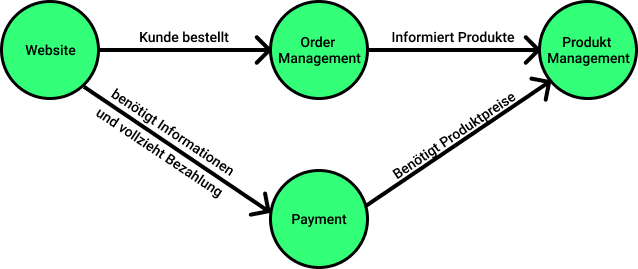
\includegraphics[width=1.0\linewidth]{img/prozess_eCommernce.png}
	\caption[Prozess Online-Shop]{Vereinfachter Prozess eines Online-Shops mit vier Komponenten\\ Quelle: Eigen}
	\label{fig:prozess_online_shop}
\end{figure}

In Abbildung \vref{fig:prozess_online_shop} ist der Prozess beschrieben. Es wird dabei nur ein einfacher Bestellprozess betrachtet. Ein Kunde bestellt auf einer Website bestimmte Produkte. Im Order-Management werden dann die Informationen zu entsprechenden Produkte, die zu dieser Bestellung gehören aus dem Produkt-Management angefordert. Mithilfe der Produktinformationen kann dann im Bezahlbereich ein Endpreis für den Nutzer kalkuliert werden. Die dort generierten Informationen können dann wieder der Website zur Verfügung gestellt werden, damit der Nutzer einen Bezahlvorgang einleiten kann.

\subsection{Monolithen}
Wird nun ein Entwicklerteam damit beauftragt ein System auf Basis dieses Prozesses zu implementieren so kann ein \textbf{monolithischer Ansatz} gewählt werden. Eine ebenfalls vereinfachte Architektur könnte für den oben beschreibenen Prozess folgendermaßen aussehen:

\begin{figure}[h]
	\centering
	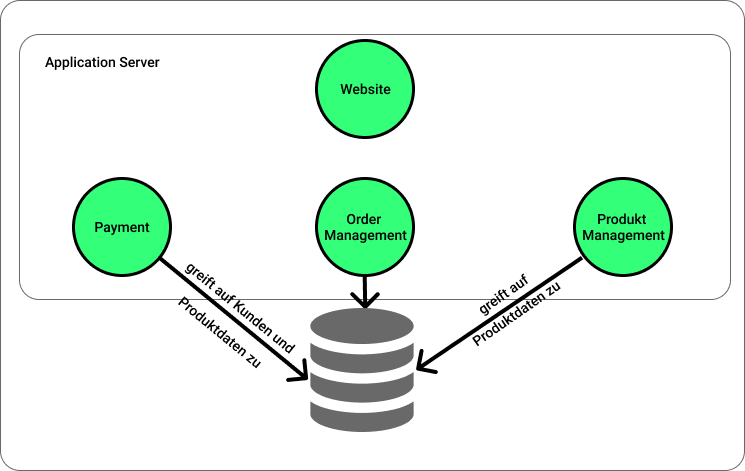
\includegraphics[width=1.0\linewidth]{img/monolitische_architektur.png}
	\caption[monolitische Architektur]{Abbildung des Prozesses mithilfe eines monolithischen Ansatzes\\Quelle: Eigen}
	\label{fig:monolithic_arch}
\end{figure}

Die in \vref{fig:monolithic_arch} beschriebene Architektur hat einige Eigenschaften, welche sie zu einer monolithischen Architektur werde lassen. Dazu gehört unter anderem die Tatsache, dass der Prozess in verscheidene Komponenten oder Module unterteilt wird, welche alle zusammen die Applikation bilden. Zusätzlich greifen alle Komponenten, da sie als eine Einheit deployt werden auf dieselbe Datenbank zu. Sowohl die Tatsache, dass es nicht in einzelne Services sonder Komponenten unterteilt wurde und das sich eine gemeinsame Datenbank geteilt wird stellen Merkmale dar, welche auf eine monolithische Architektur schließen lassen. Ein Vorteil dieses Ansatzes ist, dass die Kommunikation zwischen den verscheidenen Komponenten sehr einfach ist, da diese meistens auch logisch als \textit{ein Programm} ablaufen. So kann das Order-Management Daten anfordern indem es eine Methode im Produkt-Management aufruft. Ein \textbf{Nachteil} dieses Ansatzes besteht aber darin, dass eine sehr starke Kohäsion und Abhängigkeit von der spezifischen Implementierung einer Komponente besteht. So kann beispielsweise das Order-Management nur ausgestausch werden, wenn unter viel Aufwand auch alle anderen Komponenten in dem Monolithen angepasst werden. 

\begin{definition}[Monolith]
	Monolithen lassen sich anhand folgender Eigenschaften definieren: \autocite[S. 3]{microservice_enterprise}
	\begin{enumerate}
		\item Monolithen werden als einzelne Einheit entworfen, entickelt und deployt. Dies bringt mit sich, dass sie oftmals eine enorme Komplexität erreichen, welche nicht gut zu überblicken ist.
		\item Die einzelnen implementierten Businessfunktionen können nicht einzeln skaliert oder aktualisiert werden. Alle Komponenten sind also an zentrale Deployments des gesamten Monolithen gebunden, auch wenn nur eine Komponente aktualisiert werden muss.
		\item Die initiale Wahl einer Programmiersprache kann später nichtmehr oder nur sehr schwer wieder geändert werden, da jede einzelne Folgeentscheidung auch auf Basis dieser Wahl getroffen wurde.
		\item Bei Instabilität einer einzelnen Komponenten besteht Gefahr, dass die gesamte Applikation einen Fehler erleidet und nichtmehr funktionsfähig ist.
	\end{enumerate}
\end{definition}

\subsection{SOA und ESB}

Eine Lösung für die Nachteile, die ein Monolith mit sich bringt sollte mithilfe der \ac{SOA} erreicht werden. Die \ac{SOA} versucht die große, schwer skalierbare und stark zusammenhängende Einheit eines Monolithen aufzubrechen in kleine \enquote{self-contained} Services. Diese Services haben einen klar definierten Aufgabenbereich und besitzen ein wohldefiniertes Interface, welches \textbf{unabhängig} von der unterliegenden Implementierung ist. Dies löst bereits mehrere Probleme, welche in einem Monolithen vorhanden waren. So kann nun durch die lose Kopplung zwischen den Services (Komponenten in dem Monolithen) eine individuellere Skalierbarkeit erreicht werden. Jetzt stehen aber nicht mehr nur ein zentraler Endpunkt wie bei dem Monolithen zur Verfügung der von einem Client angesprochen werden kann. Es kommt auch die Frage auf, wie bestimmt werden kann, welcher Instanz eines Service angesprochen wird, wenn dieser in mehreren Replikaten vorliegt. Um unter anderem diese zwei wichtigen Punkte zu lösen wird die \ac{SOA} meistens nur in Verbindung mit einem \ac{ESB} verwendet.

Unter einem \ac{ESB} kann man sich vereinfacht eine Art intelligenten Load-Balancer vorstellen. Zu den klassischen Aufgaben eines \ac{ESB} gehören unter anderem die Weiterleitung der Anfragen eines Clients zu den richtigen Services. Der Grund warum es sich bei dem \ac{ESB} um einen Art intelligenten Load-Balancer handelt ist, weil er zusätzlich die Fähigkeit besitzt einzelne Services zu zusammengesetzten logischen Einheiten zu kombinieren. Wie diese Services kombiniert werden obliegt dabei dem Implementierenden, welcher es auf Basis des zu implementirenden Prozesses entscheiden kann. Zusätzlich können in einem \ac{ESB} noch Funktionen wie beispielsweise Authenthifizierung von Clients oder auch Monitoringfunktionen eingebaut werden.\\
Das oben eingeführte Beispiel könnte umgesetzt in einer \ac{SOA} folgendermaßen umgesetzt werden:
\begin{figure}[]
	\centering
	\caption{TODO: Hier kommt noch das Bild der SOA Arch hin}
\end{figure}

Diese nächste \enquote{Entwicklungsstufe} auf dem Weg zur Microservicearchitektur lässt sich also mithilfe folgender Eigenschaften definieren:

\begin{definition}[SOA und ESB]
	Im Rahmen der \ac{SOA} ist ein Service mit folgenden Eigenschaften definiert: \autocite[S. 4]{microservice_enterprise}
	\begin{enumerate}
		\item Ein Service ist eine eigenständige Implementierung einer wohldefinierten Businessfunktion, welcher über das Netzwerk erreichbar ist. Sie sind lose gekoppelt und verfügen über ein wohldefiniertes Interface über welches sie nach außen hin ansprechbar sind, somit sind sie implementierungsunabhängig. Services stellen die Grundbausteine innerhalb der \ac{SOA} dar.
		\item Zusammengesetzte Services können mithilfe auf Basis bestehender Services generiert werden und erben alle Eigenschaften, die ein Service auch hat.
		\item Services können dynamisch registriert werden. Es ist oftmals für den Client nicht von relevanz den genauen Ort eines Services zu kennen, da diese im Rahmen einer Service-Registry in Form von Metadaten vorliegen.
	\end{enumerate}
	Dem \ac{ESB} fällt dabei die Rollen eines intelligenten Mittelsmann (\enquote{smart Pipeline}) zu. Er besitzt die Möglichkeit Services zusammenzufassen und sich um die Sichtbarkeit, sowie die zusätzliche Bereitstellung von Funktionen zu kümmern. Er stellt einen zentrale Schnittstelle zwischen den einzelnen Services und der \enquote{Außenwelt} innerhalb der \ac{SOA} dar.
\end{definition}

\subsection{Der letzte Schritt - die Microservicearchitektur}

%%%%%%%%%%%%%%%%%%%%%%%
%	OBSERVABILITY	  %
%%%%%%%%%%%%%%%%%%%%%%%
\section{Observability}

Der Begriff und der Nutzen von Observability für Services lässt sich anhand der folgenden Zitate sehr gut nachvollziehen.

\begin{quote}
	\enquote{Collecting data is cheap, but not having it when you need it can be expensive.}\autocite[S. 373]{microservice_enterprise} - \textit{\citeauthor{microservice_enterprise}}

	\enquote{Observability is the measure of how well internal states [...] of a system can be inferred by knowledge of its external outputs [...].}\autocite[S. 35]{Yordanova2016} - \textit{\citeauthor{Yordanova2016}}
\end{quote}

Innerhalb einer jeden Technologie wird uns durch Standards \marginpar{CNCF} eröglicht wichtige Einsichten in Services zu erhalten. Wird jedoch darauf verzichtet Daten aus einem Service zu sammeln, so kann es im Fehlerfall die Konsquenz haben, dass Fehler erst garnicht entdeckt oder bemerkt, geschweige denn gelöst werden. Die Observability von Services, welche innerhalb einer Applikation genutzt werden ist also von essenzieller Bedeutung. Nun kommt die Frage auf, was genau ist Observability? Welche Aspekte meines Service muss ich überwachen, um zuversichtlich sien zu können, einen Fehlerfall schnell bemerken zu können und diesen dann durch die gesammelten Daten schnell analysieren zu können?\\
In \citetitle{Sridharan2018} wird beschrieben, wie sich Services in verteilten Systemen observieren lassen. Dazu nimmt der Autor eine Unterteilung in drei Säulen vor.

\begin{definition}[Die drei Säulen der Observability]\autocites[Chapter 4: Three Pillars of Observability]{Sridharan2018}[S. 373f]{microservice_enterprise}
	Um erfolgreich auf interne Zustände schließen zu können, müssen Daten existieren auf deren Basis Schlussfolgerungen gezogen werden können. Diese Daten werden aus drei verschiedenen Bereichen erhoben:

	\newcounter{pillarsCounter}

	\begin{enumerate}
		\item \textbf{Logging:}\\
		Das Zeil des Loggings besteht darin, Ereignisse zu dokumentieren. Es ist dabei nicht von Bedeutung, um welche Events es sich handelt. Zusätzlich zu den eigentlichen Daten des Ereigisses, welche unterschiedlichster Art sein können, ist es möglich Metadaten zu loggen, welche dem Ereigis zusätzlichen Kontext verleihen oder einen sonstigen Mehrwert bieten. Dazu gehören z.B. Information zum Zeitpunkt des Ereigisses (\textit{timestamp}), Ergebnis des Ereigisses (\textit{status}), usw. 
		
		Ein Vorteil des Loggings bestehen unter anderem darin, dass diese extrem einfach zu generieren sind. Ein Nachteil des Loggings besteht darin, das Logs an sich keine zusätzliche Aussagekraft haben, außer ihrem direkten Inhalt. Es ist schwer rein anhand von Logs ein komplexes Fehlerbild in einem verteilten System zu finden und korrekte Maßnahmen zur Behebung zu treffen.
		\item \textbf{Metriken:}\\
		Metriken stellen eine numerische representation von Daten dar, welche über bestimmte Zeitintervalle gemessen wurden. Metriken können also als Indikator verwendet werden, wie gut oder schlecht ein Services performt. Populäre Metriken wären z.B. die Anzahl der Anfragen, die ein Service in einer Minute verarbeitet, oder die durschnittliche Antwortzeit eines Service (seine Latenz). Das zweite Beispiel zeigt sogar ein Zusammenspiel zwischen zwei Säulen auf. Diese Metrik kann als abgeleitete Eigenschaft aus Daten des Loggings interpretiert werden, da die Latenz als Differenz zwischen dem Zeitpunkt der Anfrage und dem Zeitpunkt der Antwort ist.
		\setcounter{pillarsCounter}{\value{enumi}}
	\end{enumerate}

	\textbf{Logging} kann also als datenaggregierende Säule angesehen werden. \textbf{Metriken} hingegen nutzen (unter anderem) die aggregierten Daten, um neue wertvollere Informationen abzuleiten. Die Kombination zwischen diesen beiden Säulen bietet einem Aussenstehenden einen guten Einblick in den internen Zusatand \textit{eines} Services. Wie bereits bei der Defintion eines Microservices erwähnt ist es aber nicht unüblich hunderte kleine Services beobachten zu müssen. Es wäre allerdings sehr unpraktisch nur die einzelnen Services in Isolation zu betrachten, da es sich um stark vernetzte und voneinander abhängige Services handelt. Deshalb existieren noch eine dritte Säule, um auch serviceübergreifend Daten zu aggregieren und diese zu verwertbaren Informationen umzuwandeln.

	\begin{enumerate}
		\setcounter{enumi}{\value{pillarsCounter}}
		\item \textbf{Tracing:}\\
		Betrachtet man die bisherigen Säulen, so lässt sich ein Trend auf der Betrachtungsebene feststellen. Das Logging fokussiert sich auf die Sammlung der Daten einzelner Ereignisse, der kleinsten Einheit. Die Metriken arbeiten nun ereignisübergreifend und wandeln die Daten zu nutzbaren Informationen um, damit Einsichten in das Verhalten eines Services vorhanden ist - die mittlere Einheit. Der nächste logische Schritt wäre nun, da Services in einem verteilten System miteinander vernetzt sind, eine Anfrage von Beginn bis zur endgültigen Antwort serviceübergreifend zu observieren, quasi eine End-to-End Betrachung. Genau diese Betrachtung wird mithilfe von Tracing ermöglicht. Eine \textit{Trace} (\enquote{Spur}) ist eine Liste zusammenhängender, verteilter Eregnisse, welche als Repräsentant einer End-to-End Anfrage angesehen werden können.
	\end{enumerate}

\end{definition}
Mithilfe dieser drei Säulen ist es nun einem Aussenstehenden möglich auf \enquote{die inneren Zustände eines Systems auf Basis seiner Ausgaben} zu schließen. Dazu ein kurzes Beispiel:\\
Es wird ein Fehler bei einer Anfrage regisitriert. Der dafür zuständige Mitarbeiter kann nun mithilfe des \textbf{Tracings} feststellen um welches Request es sich handelt. Dabei erkennt er, welche Services als Ursache für den Fehler infragekommen. Im nächsten Schritt kann er sich einzelne \textbf{Metriken} der Services ansehen, um eventuell eine Anomalie festzustellen. Im letzten Schritt kann er durch ansehen der \textbf{Logs} eine genaue Fehlerursache feststellen.


\section{Gouvernance}

Eine Einführung von Microservices in ein Unternehmen kann sehr viele Vorteile besitzen. Sollte sich ein Unternehmen dazu entschließen, von der bisherigen Architektur auf eine Microservicearchitektur umzustellen, bringt dies auch einige Herausforderungen mit sich. Sind in einem Unternehmen bisher nur Monolithen bekannt, so kann die durch Microservices hinzukommende Komplexität schnell zu einem Problem werden. Zumal es sich hierbei um eine immense Anzahl neuer Services, am Beispiel von Netflix sogar mehr als 700 handeln kann. Es stellt sich nun also auch aus der Sicht eines Unternehmens die Frage, wer ist zuständig für einen bestimmten Service? Wie hängen die Services zusammen? Welche Services sind überhaupt vorhanden? Wie können Fehler in einzelnen Services erkannt werden und deren Auswirkungen bestimmt werden?

All diese Frage gehören zu dem Bereich der Microservice-Gouvernance und sollten sich im Vorfeld eines Umstiegs auf eine Microservicearchitektur klären lassen. In \citetitle{microservice_enterprise} wird unter der Gouvernance folgendes verstanden:

\begin{definition}[Dezentralisierte Gouvernance]
	Die dezentralisierte Gouvernance setzt sich unter anderem aus vier Kernmodulen \autocite[S. 154]{microservice_enterprise} zusammen. Dabei handelt es sich um:
	\begin{enumerate}
		\item die Observability
		\item eine Service-Registry und Service-Discovery
		\item das API-Management und
		\item die Entwicklungszyklen
	\end{enumerate}
	Diese vier Kernmodule sind innerhalb eines Microservice Ansatzes nicht dezentral verwaltbar. Weitere Bestandteile eines Microservice, welche im Bereich der Gouvernance liegen sind design, development und deployment eines Services. Hierfür sollt es keine zentrale Verwaltung geben,\autocites[S. 154]{microservice_enterprise} [Decentralized Gouvernance]{FowlerMicrservices}sonder die Veranwtortlichkeit sollte im entwickelnden Team liegen.
\end{definition}

Eine dezentralisierte Gouvernance wie sie bei Microservices genutzt wird hat einie Vorteile gegenüber dem früheren komplett zentrierten Gouvernance-Ansatz. So kann zum Beispiel für jeden Anwendungsfall die Tools von dem zuständig Team selbst gewähl werde und es wird nicht von einer unternehmensweiten Grundsatzentscheidung bestimmt, dass nur ein bestimmer Technologieverbund genutzt werden kann. Trotz dieser Freiheit bleiben wichtige Elemente wie die Observability eines Services in einem zentralisierten skalibaren Service verfügbar, sodass wichtige Daten immer von allen Services zur Verfügung stehen. Hier ist eine zentrale Vorschrift sogar förderlich, da so sichergestellt wird, dass keine \enquote{Insights} verloren gehen, da ein Subset der im Unternehmen vorhanden Service andere Tools für das Monitoring benutzen als der Rest.

Im Rahmen dieser Arbeit wird in Kaptiel \vref{chap:KonzepTool} ein Tool vorgestellt, welches ein Problem im Bereich der Gouvernance in Verbindung mit Elementen aus der Observability lösen soll. Dabei ist eine weitere zentralisiert verwaltete Komponente der Gouvernance relevant. Dabei handlet es sich eine Art Service-Registry mit erweiterter Observability Funktionalität.

\section{Betrachtung bestimmter Gesichtspunkte im Rahmen der Gouvernance und Observability}

Viele Konzepte, welche für Microservices essenziell sind stellen mit einem strengen Blick auf die Gouvernance und die Observability eine Herausforderung dar. So werden im folgenden Teil einige dieser Konzepte vorgestellt und die damit verbundenen Probleme erläutert. Diese Probleme müssen mithilfe von Tooling oder eventuell sogar Designentscheidungen während der Softwareentwicklung verhindert werden.

\subsection{Design for Failure}
Bei Design for Failure \autocite{FowlerMicrservices} handelt es sich um ein Kernprinzip, welches bereits von \citeauthor{FowlerMicrservices} in seiner Zusammenstellung zu dem Architekturprinzip Microservice in \enquote{\citetitle{FowlerMicrservices}} vorgestellt wurde. Die Idee hinter diesem Prinzip ist, dass Fehler immer, erst Recht im Softwareumfeld unvermeidbar sind. Deshalb müssen 


Design for Failure, aber wie bekomme ich es mit? Wie reagiere ich im Fehlerfall? Was muss getan werden, und wie groß sind die Auswirkungen wenn einer meiner tausend Microservices ausfällt? Diese und viele weitere Fragen müssen sich DevOps und Software-Engerneering Teams oftmals stellen, wenn sie sich in einer dezentralisierten Microservicearchitektur befinden. Es ist oftmals ein tiefes Verständnis des Zusammenspiels der einzelnen Services nötig um heruaszufinden, ob ein Fehler von eigenen Service kommt, oder ob es aufgrund eines Fehlers in einem anderen Service kommt. Das ultimative Ziel ist es dabei herauszufinden was das Problem ist und dieses auch schnellstmöglich zu beheben, sodass für den Endnutzer keine Merkbaren folgen auftreten. Microservices folgen dem Prinzip \enquote{Design for Failure}, sodass eine Recovery möglich ist und ein operatives Business aufrecht erhalten werden kann. Trotz dieser hervorragenden Prämisse reicht ein \enquote{Design for Failure} alleine nicht aus. \enquote{Ein System ist nur so schlau wie das schwächste seiner Bestandteile}. Microservices mit dem Ziel kleiner dezentralisierter Services, welche einen spezialisiert sind auf eine bestimmte aufgabe innerhalb eines BusinessProzesses haben ironischerweise eine ihrer größten Schwäche in der Kommunikation miteinander. Es müssen Standards etabliert werden, sodass ServiceOwner einen wartbaren und funktionsfähigen Service entwickeln können. Es muss einen Software-Engeneer an einer Stelle ein Fehler unterlaufen und aufgrund der starken Kohäsion und Abhängigkeit der einzelnen Services unterneinander kann eine Reihe wichtiger Businessfunktionen davon betroffen sein. Im Beipsiel von Amazon führte ein Fehler in einem Service zu einer 20 Minütigen Downtime der Verkaufswebsite, was einem monetären Verlust von ca. 3.5 Mio Euro gleichkommt.

Kein Problem - \enquote{Design for Failure}. Ein Service fällt aus und ist darauf ausgelegt sich selbst wieder zu reaktivieren. Alle anderen Services können einen ausfall händeln. Soweit die Theorie. In der Praxis ist das leider nur allzuoft nicht der Fall. Innerhalb der Microservice-Gouvernance steht der Aspekt der dezentralisierten Entscheidungsfindung im Vordergrund. Das bedeutet, dass jedes Team das fachliche und unternehmerische Know-How zugesprochen wird das beste Tool und die beste Technologie für die von ihnen zu lösende Aufgabe zu wählen. Fängt ein Architekt nun an diese Aufgabe zu lösen, so benötigt er oftmals Informationen aus anderen Microservices, um seine Aufgabe zu erfüllen. 


\begin{center}
	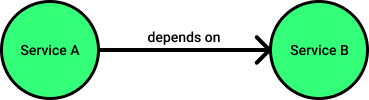
\includegraphics[width=0.55\linewidth]{img/service_dependency.png}
\end{center}

Es entsteht also eine Abhängigkeit zwischen zwei Microservices. Ebendieser angefragte Microservice benötigt aber wiederum einen anderen Service, um die angeforderte Information generieren zu können. Es entsteht also schon eine Kette von Abhängigkeiten. Was passiert, wenn ein Glied dieser Kette einen Fehler wirft? 

\Large Hier kommt ein Bild von einem Fehler in einer Microsericekette

\normalsize

Kein Problem - \enquote{Design for Failure}. Ein Architekt muss in der Planung seines Services die Möglichkeit haben, das Risiko und die Auswirkungen einen Ausfalls sowohl seines eigenen Services, als auch seiner Abhängigkeiten einschätzen zu können. Diese Einschätzung sollte auf Daten basieren, welche sowohl Information bisheriger Ausfälle und deren Ursachen enthalten als auch Ausblicke geben können auf den aktuellen Stand und eventuelle zukünftige Ausfälle.

Wie bereits Eingangs erwähnt ist bei der Betrachtung dieses Prinzips die Brille der Gouvernance und Observability aufgesetzt. Es ist ein wichtiger Bestandteil die Services innerhalb einer Unternehmensarchitektur so aufzubauen, dass diese trotz eins Fehlers ordnungsgemäß weiterlaufen und die Fähigkeit zur Recovery besitzen. Dieses Prinzip ist sogar dafür Veranwtortlich, dass Microservicepioniere wie Netflix innerhalb der Observability eine eigene, vierte Säule zu etablieren. Dabei handelt es sich um das sogenannte Chaos-Testing. Um dies kurz zu erläutern: Dabei handelt es sich um einen eigenen \enquote{Service}, welcher auf Basis von Chaos-Experimenten produktive Services ausschaltet und so die Recovery ebendieses Services und auch der davon abhängigen Services überprüfen kann. Dies bringt viele Vorteile mit sich und sorgt auch dafür, dass Services gut entwickelt sind. Diese Idee, wie das bewusste Einführen von Fehlern die generelle Qualität von Services verbessern kann, wird näher in \citetitle{AntifragileOrganization}\autocite{AntifragileOrganization} beschrieben.


\chapter{Konzeption einer graphbasierten Serviceregistry}

Im folgenden Kapitel wird versucht auf Basis der in \vref{chap:Anforderungen} beschriebenen Anforderungen ein Konzept für ein Tool zu erarbeiten, welches als \enquote{intelligente} Service-Registry fungiert. Dazu wird zunächst eine mögliche Technologiewahl erläutert. Danach werden noch einige möglichen Funktionen mithilfe von Beispielen vorgestellt.

\section{Wieso wird ein Graph verwendet?}

Bereits in \citeauthor{Ren2018} wird ein Graph verwendet, um zu beschreiben wie ein einfacher Übergang zwischen einer ehemals monolithischen Architektur zu einem Microserviceansatz erreicht werden kann. In diesem Fall wird ein Abhängigkeitsgraph verwendet, um die Zusammenhänge zwischen den verschiedenen Komponenten zu beschreiben. Anhand dieses Graphen wird dann versucht die benötigten Services zu definieren. Der Graph beschreibt also Zusammenhänge zwischen den verschiedenen Services \autocite[Kapitel 3.2 \& Kapitel 3.3]{Ren2018}. Diese Idee bildet auch das Fundament des vorgeschlagen Konzepts. Um allerdings zu verstehen, wieso ein Abhängigkeitsgraph auch als Basis für eine Serviceregistry dienen kann, muss zuerst erläutert werden, was ein Graph ist und wie Graphdatenbanken dabei helfen können, dieses abstrakte Modell für die Softwareentwicklung nutzbar zu machen.

\begin{definition}[gerichteter Graph]\autocite[Kapitel 1.2]{Bang-Jensen2007}
	Ein gerichteter Graph ist ein geordnetes Tupel $$G = (V,A)$$ für das gilt:
	\begin{itemize}
		\item $V(G)$ ist eine nichtleere Menge, deren Elemente man Knoten (engl. \textit{verticies}) nennt
		\item und einer endlichen Menge $A(G) \subseteq V \times V$ von geoordneten Tupeln verschiedener Knoten, die man Kanten (engl. \textit{arcs}) nennt.
	\end{itemize}

	Bei einem gerichteten Graphen handelt es sich um ein \textbf{geordnetes Tupel} $v \in A$, wobei die \enquote{Richtung} vorgegeben ist durch die Reihenfolge im Tupel. Bei einem ungerichtetetn Graphen besteht $A$ aus einer Menge \textbf{ungeordneter Tupel}.
\end{definition}

Diese mathematische Definition beschreibt eine interessante Datenstruktur für die Informatik und die Softwareentwicklung. Diese Datenstruktur versucht also die vorgegebenen Eigenschaften eines Graphen, wie in der Graphentheorie beschrieben, zu realisieren. \\
Eine Unterkategorie bei den gerichteten Graphen sind sowohl zyklische, als auch azyklische gerichtete Graphen. Dabei handelt es sich um Repräsentaten eines gerichteten Graphen, welche keinen gerichteten Kreis enthalten. Betrachtet man nun den Anwedungsfall des zu konzeptionierenden Tools, so stellt man fest, dass ein azyklischer Graph nicht die richtige Wahl wäre. Dies soll im Folgenden erläutert werden.

\begin{example}
	Beginnen wir mit der formalen Definitionen des Graphen, welcher die Beziehung zwischen Microservices abbilden soll. Der Graph $G$ besteht dann also aus: 
	\begin{itemize}
		\item der Menge $V(G)=\text{Menge aller Services in einem Unternehmen}$
		\item der Menge $A(G)=\{a,b \mid \text{a benötigt Informationen aus b}\}$
	\end{itemize}
	Der Graph beinhaltet also Informationen über einen Service, als auch über seine Verbindungen mit anderen Services. Da es ein gerichteter Graph ist gilt für $$(a,b), (b,a) \in A(G),\text{ dass }(a,b) \neq (b,a),$$ da es sich bei den Elementen von $A(G)$ um geordnete Tupel handelt. Diese Tatsache spiegelt sich auch in der Realität wieder, da die Abhängigkeit eines Services $a$ von einem Service $b$ nicht dieselbe Anfrage widerspiegelt, die Service $b$ von Service $a$ hat.
\end{example}\label{exp:microserviceGraph}

Man erkennt also bereits jetzt, dass rein mit dem mathematischen Modell eines Graphen bereits viele realen Aspekte übereinstimmen, was es als potenzielles Datenmodell qualifiziert. Die Datenstruktur eines Graphen hat zusätzlich noch die Möglichkeit Informationen sowohl an den Knoten, als auch an den Kanten zu speichern \footnote{TODO: Quelle}. Zusätzlich könnte eine weitere Idee aus der \textbf{Graphentheorie} eine nützliche Ergänzung zu der bisherigen Idee darstellen.

\begin{definition}[Fluss]
	In der Graphentheorie stellt ein Fluss eine Funktion $f: A \rightarrow \mathbb{R_+}$ dar, die jeder Kante $a \in A(G)$ einen nichtnegativen Flusswert $f(a) \in \mathbb{R_+}$ zuweist. Des Weiteren muss folgende Bedingung erfüllt sein, damit es sich bei dieser Funktion um einen Fluss handelt. Dafür muss gelten, dass der Flusswert einer Kante $a \in A(G)$ höchstens so groß ist, wie die Kapazität der Kante mit: \footnote{TODO: Quelle, Netzwerk noch erklären} $$\forall a \in A(G): f(a) \leq u(a)$$
\end{definition}

Mithilfe der Idee einer Flussfunktion in einem Graphen können die Kanten und die Beziehungen zwischen den einzelnen Services genauer dargestellt werden. Die Gewichtung der Kanten kann eine Repräsentation der Intensität der Nutzung dieser Kante darstellen.

Dieses mathematische Model beschreibt das zu lösende Problem bereis sehr gut. Deshalb ist es sinnvoll als Datenstruktur zur Abbildung der Daten einen Graphen zu wählen. Graphen können auf technischer Ebene auf verschiedenste Weise implementiert werden. Die Entscheidung welcher Implementierung am sinnvollsten ist, soll aber im Rahmen dieser Arbeit nicht getroffen werden. Einer der populärsten Datenbanken im Bereich der Graphdatenbanken stellt Neo4j dar. Diese Datenbank folgt dem Prinzip der \enquote{index-free adjencency}, was soviel bedeutet wie, dass benachbarte Knoten auch nebeneinander persistiert werden, sodass bei einem Lesevorgang auf das kostspielige Auswerten von Indices verzichtet werden kann. So können auch große Graphen von einer sehr schnellen Lesezeit profitieren. Gleichzeitig kann dieses \ac{DBMS} mithilfe der populären Abfragesprache \texttt{CYPHER} genutzt werden.

\section{Bewertung einer alternativen Methode}

Im folgenden Abschnitt wird eine Methode vorgestellt, welche versucht das gleiche Problem zu lösen, wie das in der Arbeit präsentierte Konzept. Dabei wird versucht verschiedene Komponenten der Firma Elastic zu kombinieren, um eine Lösung zu konstruieren. Elastic ist unter anderem bekannt durch das Produkt ElasticSearch, welches ein dokumentenbasiertes \ac{DBMS} ist.

\begin{figure}[h]
	\centering
	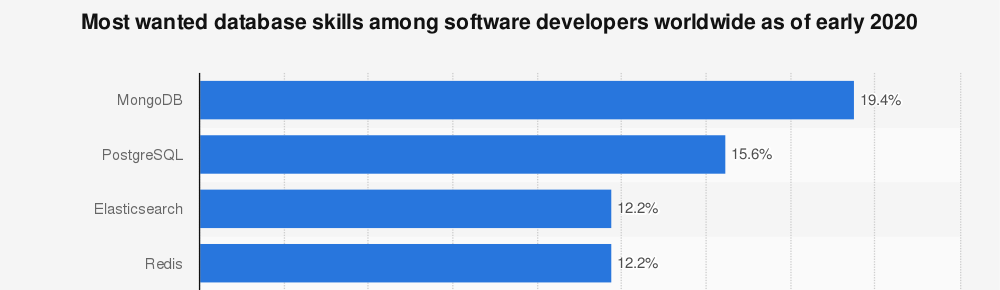
\includegraphics[width=1.0\linewidth]{img/statista_db.png}
	\caption{Stack Overflow. "Most wanted database skills among software developers worldwide as of early 2020." Chart. February 15, 2020. Statista. Accessed August 18, 2020. \url{https://www.statista.com/statistics/793854/worldwide-developer-survey-most-wanted-database/}}
\end{figure}

ElasticSearch erreicht eine sehr gute Suchperformance durch das Verwenden von Indizes und einer guten Tokenisation der indizierten Daten. Zusätzlich ist ElasticSearch so aufgebaut, dass es einfach innerhalb eines Clusters verwendet werden kann. Die in einem Cluster vorhandenen Nodes können auf verschiedenste Weisen konfiguriert werden. Innerhalb von ElasticSearch gibt es auch die Möglichkeit \ac{ML} Funktionen zu verwenden. Diese \ac{ML} Funktionen sind die Grundlage für das Konzept, welches das Problem lösen könnte. Dazu werden, zusätzlich zu \ac{ML}-Nodes noch andere Produkte der Firma Elastic verwendet.

Ein weiteres Produkt nennt sich \ac{APM}\footnote{\url{https://www.elastic.co/de/apm}}, welches die Möglichkeit hat sowohl anwedungsspezifische Daten, als auch hardwarespezifische (oder containerspezifische) Metriken zu sammeln und direkt in einen entsprechenden ElasticSearch-Index zu speichern. Für das \ac{APM} gibt es Integrationen für alle wichtigen Programmiersprachen\footnote{\url{https://www.elastic.co/guide/en/apm/get-started/current/index.html}}. Diese Software liefert wichtige Informationen über den aktuellen Zustand eines Services und bietet auch gleichzeitig eine zentralisierte Sammelstellen für diese Metriken. 

Dies erfüllt die Punkte vier und fünf der Anforderung \vref{chap:Anforderungen}. Das initiale Aufsetzen der Infrastruktur benötigt allerdings durchaus produktspezifisches Know-How. Danach ist es aber ein sehr einfacher Prozess neue Services anzuschließen, da dies rein auf Serviceebene, also von den implementierenden Teams erledigt werden kann und unterstützt somit den dezentralen Ansatz einer Microservicearchitektur. Es fehlt allerdings noch die Auswertung und Aufbereitung der durch \ac{APM} gesammelten Daten. Dazu kann das Visualisierungstool von Elastic, \textbf{Kibana}\footnote{\url{https://www.elastic.co/de/kibana}}, verwendet werden. \\
Kibana nutzt die vorhandenen Indizes in einem ElasticSearch Cluster, um verschiedenste Operationen, meistens visualisierender Art, durchzuführen. Dort können auch eigene Visualisierungen konfiguriert werden, welche dem Endnutzer ermöglichen, eine für ihn optimale Informationslandschaft zu gestalten. Dies erfüllt das zweite definierte Kriterium aus \vref{chap:Anforderungen}, da es die durch \ac{APM} gesammelten Daten zu wertvollen Informationen aufbereitet, welche Hinweise geben auf den internen Zustand eines Services.

Die Kombination aus \ac{APM} und Kibana stellen also Tools dar, die einen Fokus auf die Observability haben. Das eigentliche Problem beinhaltet aber auch, dass ein Nutzer sehr schnell wissen muss, um welchen Fehler es sich handelt und wie groß die Auswirkungen davon sind. Zusätzlich ist es wichtig, bereits während der Entwicklung eines Services zu wissen, in welcher Umgebung sich der Service befindet. Um diese Governanceaspekte in diesen Lösungsvorschlag zu integrieren kommen die bereits angesprochenen \ac{ML} Nodes ins Spiel. Diese bieten die Möglichkeit eine Analyse der Daten in einem Index durchzuführen. Ab dann kann festgestellt werden, ob ein System \enquote{normal} operiert oder nicht. Sollten nun Metriken aus \ac{APM} in dem Index gespeichert werden, welche Hinweise auf einen Fehler enthalten, so wird die Analyse dies erkennen und besteht die Möglichkeit des schnellen Entdeckens des Fehlers. Gleichzeitig beinhaltet die Nutzung der \ac{ML} Funktionalität auch einige Schwierigkeiten.

So ist es z.B. während der Analyse schwer zu unterscheiden, ob eine erkannte Anomalie wirklich ein Fehler ist, oder einfach nur ein neuer Service, der hinzugefügt wurde. Es ist auch nur schwer möglich die Metriken unterschiedlicher Services in einer einzelnen \ac{ML} Node auszuwerten, da durch unterschiedliche Hardwaredaten der verschiedenen Services ein sehr breites Spektrum als \enquote{normal} angesehen wird. Es gilt also hierfür eine Lösung zu finden, welche nicht beinhaltet, dass für jeden neuen Service eine neue \ac{ML} Pipeline angelegt werden muss.

Die Idee dieses bestehenden Tools zu verwenden, um das Problem zu lösen ist prinzipiell nicht von der Hand zu weisen, da auch einige wesentliche Anforderungen aus \vref{chap:Anforderungen} erfüllt werden. Allerdings bringt es auch Schwierigkeiten mit, die es vor der Einführung und dauerhaften Nutzung dieser Tools zu lösen gilt.

\section{Konzept unter Nutzung einer Graphdatenbank}

Im ersten Abschnitt dieses Kapitels wurden bereits Grundlage im Bezug auf Graphen und deren Eigenschaften erläutert. Die Idee Graphen zu verwenden, um Abhängigkeiten und Verbindungen zwischen Elementen darzustellen ist nicht neu \autocite{Ren2018}. Bereits \citeyear{Metayer1998} erläuterte \citeauthor{Metayer1998} in \textit{\citetitle{Metayer1998}} einen Ansatz, wie man mithilfe formaler Sprachen die Softwarearchitektur in einem Graphen abbilden kann \autocite{Metayer1998}.

\begin{example}[Abhängigkeitsgraphen]
	Abhängigkeitsgraphen werden auch in Toolings für verschiedene Programmiersprachen verwendet. Ein Beispiel ist JavaScript. Diese ermöglichen es Dateien, verschiedenen Formats miteinander zu kombinieren und in einer Datei, dem Bundle, zusammenzuführen. Dabei ist es wichtig, dass alle Dateien in der richtigen Reihenfolge in das Bundle integriert werden, um am Ende ein lauffähiges Programm zu erhalten. Um zu wissen, welche Dateien in welcher Reihenfolge eingefügt werden müssen, wird ein Abhängigkeitsgraph erstellt, an dem abgelesen werden kann, welche Datei benötigt wird, um eine andere valide Datei zu erhalten.
\end{example}

Das Konzept eines Abhängigkeitsgraphen ist auch die Grundlage für die Idee, die Abhängigkeiten zwischen Services über einen Graphen darzustellen. Für die Realisierung des Konzeptes kann eine beliebige Graphdatenbank gewählt werden. Dabei sollte aber darauf geachtet werden, dass es sich um eine \enquote{native} Graphdatenbank handelt. Das bedeutet, dass der primäre Anwedungsfall des \ac{DBMS} die Darstellung und Speicherung der Daten in einem Graphen ist. Andere \ac{DBMS}, wie z.B. Elastic oder MongoDb bieten auch die Möglichkeit Daten mithilfe von Graphen darzustellen und zu speichern. In diesen Datenbanken sind die Graphen nur unter Zuhilfenahme einer großen Anzahl an Indizes realisierbar \autocite{JoyChao2016}. Diese \enquote{nicht-nativen} Graphen haben oftmals eine deutlich schlechtere Performance als ein \ac{DBMS}, welches einen nativen Graphen realisiert.\\
Für den oben beschriebenen Anwendungsfall sollte also ein \ac{DBMS} gewählt werden, welche eine native Implementierung eines Graphen besitzt.

\subsection{Das Konzept einer graphbasierten Service-Registry}

Wie bereits in Beispiel \vref{exp:microserviceGraph} beschrieben, kann die Menge der Knoten in einem Graphen mit den Microservices innerhalb eines Unternehmens gleichgesetzt werden. Diese Knoten können mithilfe einer Graphdatenbank noch zusätzliche Eigenschaften erhalten. Im folgenden wird exemplarisch \textbf{Neo4j}\footnote{\url{https://neo4j.com/}} als Repräsentant eines graphbasierten \ac{DBMS} verwendet. Allerdings können sind die genutzten Funktionen auch in anderen Graphdatenbanken verfügbar.

Die grundlegende Idee soll anhand eines sehr einfachen Graphen beschrieben werden. Dieser Graph $G$ ist definiert mit:
\begin{itemize}
	\item $V = \{\text{Service A, Service B}\}$ und
	\item $A = \{(\text{Service A},\text{Service B}), (\text{Service B}, \text{Service A})\}$
\end{itemize}

Diese Defition führt zu folgenden Graphen:

\begin{figure}[h]
	\centering
	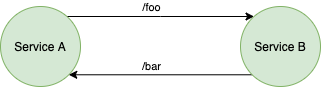
\includegraphics[width=0.65\linewidth]{img/service_dependencies.png}
	\caption[Abbildung eines simplen Abhängigkeitsgraphen]{Visualisierung des Graphen\\Quelle: Eigen}
\end{figure}

Da es sich um einen gerichteten Graphen mit geoordneten Tupeln als Elemente der Kantenmenge $V$ handelt, kann die Richtung der Abhängigkeit erkannt werden. Zu lesen ist es folgendermaßen:

\begin{center}
	Service A benötigt den \texttt{/foo}-Endpunkt von Service B\\
	Service B benötigt den \texttt{/bar}-Endpunkt von Service A
\end{center}

In der mathematischen Darstellung alleine ist allerdings noch keine Information bzgl. der Abhängigkeit zu erkennen. In einem \ac{DBMS} wie Neo4j ist dies allerdings möglich, da es dort möglich ist sowohl an Knoten (Nodes), als auch an Kanten (Relations) Schlüssel-Wert Paaren zu speichern \footnote{\url{https://neo4j.com/developer/graph-database\#property-graph}}. Dies ermöglicht einer Service-Registry die benötigten Metadaten zu speichern, sowohl um die Services an den Knoten, als auch um die Abhängigkeiten näher zu beschreiben.

\subsection{Mögliche Realiserungen des Konzepts}

Im Folgenden werden verschiedene Ansätze präsentiert, welche versuchen, die durch das Datenmodell geschaffenen Möglichkeiten, so umzusetzen, dass eine den in \vref{chap:Anforderungen} beschriebenen Anforderungen entspricht.\\ Um eine den Anforderungen gerechte Service-Registry entwickeln zu können, werden zwei Komponenten benötigt. Zum einen, auch der Kernbestandteil, wird eine \textit{zentrale Komponente} benötigt, die Funktionen einer Service-Registry realisiert. Das bedeutet, sie muss alle Services kennen und auch deren Beziehung zueinander darstellen. Es stellt sich nun die Frage, wie die Informationen über Art und Zusammenhang der Services zu der zentralen Komponente gelanden. Dazu werden zwei Verfahren vorgestellt:

\subsubsection*{1. Statischer Ansatz}
Wie bereits in der Definition eines Microservice festgehalten, ist es in der Pflicht des dafür zuständigen Teams parallel zum Service auch eine \textbf{Service Defintion} bereitzustellen. Dafür können die schnittstellenspezifischen Standards genutzt werden. Ein offener Standard zum beschreiben von REST Schnittstellen ist OpenAPI 3.0\footnote{\url{https://swagger.io/specification/}}. REST oder RESTful Services sind die aktuell meistgenutzen Formate bei Webservices. Innerhalb dieses Standards gibt es außerdem die Möglichkeit, weitere Metadaten zum beschreiben eines Services zu speichern. Um dem Graphen die benötigten Daten bereitzustellen, kann das für einen Service zuständige Team die Abhängigkeiten in ein speziell definiertes Metadatenfeld eintragen\footnote{\url{https://swagger.io/docs/specification/openapi-extensions/}}. Die zentrale Komponente, die dafür verantwortlicht ist den Graphen aufzubauen, könnte dann auf Basis dieser Informationen einen die Architektur repräsenierenden Graphen konstruieren. 

Dabei wird für jede eingelesene Service Defintion ein neuer Knoten im Graphen angelegt. Es kann dann auf Basis von eigenen Identifiern oder von den angegebenen URL's bei den Abhängigkeiten dann eine Kante zwischen dem neu erstellten Service und der Abhängigkeit erstellt werden.

% TODO: Evtl. noch den Algorithmus zum auslesen und konstruieren eines Graphen reinhauen oder ein Bild von nem neo4j graphen der sowas repräsentiert

Diese Methode bringt allerdings einige Probleme mit sich, welche die Nutzung einer solchen Service-Registry erschweren würden:

\begin{enumerate}
	\item Durch den statischen Ansatz besteht die Notwendigkeit, Informationen über den eigenen Service, sowie über dessen Abhängigkeiten manuell in einem Dokument zu hinterlegen. Dies erhöht das Fehlerpotenzial immens, da sehr viele nicht automatisierte Schritte durchgeführt werden müssen. Zusätzlich müssen die Abhängigkeiten, sollten diese sich ändern, manuell in dem Dokument angepasst werden.
	\item Des weiteren stellt sich die Frage, woran ein Service identifiziert werden kann. In dem Beispiel wurde mithilfe eines extra Feldes \texttt{x-service-identifier} versucht eine eindeutige Identifizierbarkeit zu gewährleisten. Diese Methode hat allerdings mehrere Schwachstellen. Es muss entweder vor einen Servicedeployment sichergestellt werden, dass die Service-ID einzigartig im zu untersuchenden Bereich ist, oder das Deployment muss von der Service-Registry verhindert werden, solange bis ein einzigartiger Identifier gewählt wurde. Beide Varianten sind nicht nutzerfreundlich und mit einem zu hohen aufwand verknüpft.
	\item Die beiden vorherigen Probleme führen dazu, dass das Deployment eines Services nun nichtmehr einfach und im Rahmen einer agilen Entwicklung erfolgen kann, da nun ein sehr hoher administrativer Aufwand damit verbunden ist. Auch kann eine Aktualisierung des Graphen, der als Repräsentant der Service-Registry dient, nur dann erreicht werden, wenn eine neue Version der Service-Definition vorhanden ist. Dieser Ansatz widerspricht der eigentlichen Anforderung, das Fehlerrisiko so gering wie möglich zu halten.
	\item Es ist außerdem nicht möglich, zu erkennen wie stark die Abhängigkeit ist. Das bedeutet, bricht der Service komplett zusammen, da es eine notwendige Abhängigkeit ist, die sehr oft genutzt wird, oder besteht eher ein geringeres Risiko, da die Verbindungen nur sehr selten genutzt wird.
\end{enumerate}

\subsubsection*{2. Dynamischer Ansatz}

Aus den Problemen der statischen Methode lässt sich erkennen, dass viele Prozesse automatisiert ablaufen müssen. Dazu zählen unter anderem:

\begin{enumerate}
	\item die Service-Discovery,
	\item das automatische hinzufügen und aktualisieren in den Graphen und
	\item die Einführung einer Gewichtung, um zu erkennen wie \enquote{stark} eine Abhängigkeit zwischen zwei Services ist.
\end{enumerate}

\subsection{Die zentrale Komponente}

\section{Bewertung und Gegenüberstellung der Methoden}

\begin{itemize}
	\item Kurze Einführung in Graphdatenbanken, im speziellen Neo4j. Wieso passen die so gut? referenzieren auf Bilder und \enquote{Abhängigkeiten} Wie kann damit eine Lösung konstruiert werden?
	\begin{itemize}
		\item Statischer Ansatz $\Rightarrow$ von den Entwicklern definierte Abhängigkeiten werden in der Service-Definition angegeben. Der Graph kann aus diesen SD's erstellt werden. Hier gibt es Probleme: Manuelle Veranwtortlichkeit widerspricht eigentlicher Idee von Risikoeinschätzung, da ein neuer Fehler Mensch eingebaut wird.
		\item Automatischer Nutzungsbasierter, somit dynamischer Aufbau des Graphen. Prinzip ähnlich wie bei Prometheus (populäres Tool zum sammeln von Metriken). Konzept ähnlich wie Distributed Tracing. Dort werden alle Traces mit ihren Spans zusammengefasst und zentral ausgewertet. Kombination aus dieser Idee mit Prometheus-Ansatz sieht dann folgendermaßen aus:
		
		Jeder Service exposed einen \texttt{/traffic}-Endpoint der unstrukturierte Daten bzgl. der Netzwerkaktivität enthält. Diese können dann in einem Service der für den Aufbau des Graphen zuständig ist zu ebendiesem umgewandelt werden.
		\item Es kann zusätzlich überlegt werden, ob anstatt dieses \texttt{PULL}-Verfahrens eine Push Variante gewählt wird, welche ähnlich wie \texttt{fluentd} als Sidecar in einer Containererisierten Umgebung läuft. Die könnte dann periodisch die Netzwerkdaten pushen, wenn sie Zugriff darauf hat.
	\end{itemize}
	\item Es kann überlegt werden welche Metadaten zusätzlich im Rahmen dieses Graphen eine sinnvolle Ergänzugn bieten würden, sodass ein weiterer Mehrwert geschaffen werden kann. (Ist das noch im Rahmen der Arbeit? Kommt das eher in den Ausbilck mit ein paar Ideen?)
	\item Wie können jetzt die Sachen in dem coolen Graphen genutzt werden?
	\begin{itemize}
		\item Kurze \texttt{CYPHER-QUERIES} Aufschreiben:
		\begin{itemize}
			\item Wie finde ich affectete services raus
			\item was passiert wenn ein Service X ausfällt
			\item Was ist die Zentralste Komponente in meinem Unternehmen
			\item usw.
		\end{itemize}
	\end{itemize}
\end{itemize}

\chapter{Bewertung und Einschätzung der Arbeit, sowie Ausbilck auf künfitge Arbeiten}
%	Literaturverzeichnis
\clearpage
\ihead{}
\printbibliography[title=Literaturverzeichnis]
\cleardoublepage

% Der Anhang beginnt hier - jedes Kapitel wird alphabetisch aufgezählt. (Anhang A, B usw.)
% \appendix
% \ihead{\appendixname~\thechapter} % Neue Header-Definition

% Ehrenwörtliche Erklärung ewerkl.tex einziehen
% !TEX root =  master.tex

\clearpage
\chapter*{Ehrenwörtliche Erklärung}

% Wird die folgende Zeile auskommentiert, erscheint die ehrenwörtliche
% Erklärung im Inhaltsverzeichnis.

% \addcontentsline{toc}{chapter}{Ehrenwörtliche Erklärung}
Ich versichere hiermit, dass ich die vorliegende Arbeit
 mit dem Thema: \textit{\DerTitelDerArbeit} selbstständig verfasst und keine anderen als die angegebenen Quellen und
Hilfsmittel benutzt habe. Ich versichere zudem,
dass die eingereichte elektronische Fassung mit der gedruckten Fassung übereinstimmt.

\vspace{3cm}
Mannheim, \today \hfill \DerAutorDerArbeit



\end{document}
